% Gemini theme
% https://github.com/anishathalye/gemini
%
% We try to keep this Overleaf template in sync with the canonical source on
% GitHub, but it's recommended that you obtain the template directly from
% GitHub to ensure that you are using the latest version.

\documentclass[final, 20pt]{beamer}

% ====================
% Packages
% ====================

\usepackage[T1]{fontenc}
\usepackage{lmodern}
% \usepackage[size=custom,width=120,height=72,scale=1.0]{beamerposter}
\usepackage[size=a1,scale=1.3]{beamerposter}
\usetheme{gemini}
\usecolortheme{gemini}
\usepackage{graphicx}
\graphicspath{images}
\usepackage{booktabs}
\usepackage{tikz}
\usepackage{pgfplots}
\usepackage{lipsum}
% ====================
% Lengths
% ====================

% If you have N columns, choose \sepwidth and \colwidth such that
% (N+1)*\sepwidth + N*\colwidth = \paperwidth
\newlength{\sepwidth}
\newlength{\colwidth}
\setlength{\sepwidth}{0.025\paperwidth}
\setlength{\colwidth}{0.3\paperwidth}

\newcommand{\separatorcolumn}{\begin{column}{\sepwidth}\end{column}}

% ====================
% Title
% ====================

\title{Autonomous Landing with a DJI Spark and April Tags}

\author{Joshua Springer}

\institute[shortinst]{Reykjavík University}

% ====================
% Body
% ====================

\begin{document}

\begin{frame}[t]
\begin{columns}[t]
\separatorcolumn

\begin{column}{\colwidth}

  \begin{alertblock}{Problem Description}

    \heading{Goal}

    \begin{itemize}
      \item Autonomously land a drone on a landing pad marked with a fiducial marker.
      \item Identify the landing pad via a gimbal-mounted, monocular camera that tracks the fiducial marker (to increase detection range).
      \item Distinguish between multiple landing pads and actively choose one for landing.
      \item Search for landing pads safely if one is not yet found.
    \end{itemize}

    \heading{Key Background Points}

    \begin{itemize}
      \item Landing is a hard part of autonomous drone flight because it is risky and requires high precision.
      \item GPS alone does not provide a sufficiently accurate position estimate for landing.
      \item Fiducial markers can allow a drone to recognize a landing pad cheaply and accurately, unlike GPS.
      \item Previous methods have used a fixed, downward facing camera to identify fiducial markers on a landing pad,
            with the disadvantage that they can easily lose track of it.
    \end{itemize}

    \heading{Contribution}

    In this project, the gimbal-mounted camera tracks the landing pad,
    giving the advantage that the drone doesn't lose sight of the landing pad easily,
    but with the disadvantage that the drone must accurately detect not only the position,
    but also the orientation of the landing pad.
    The orientation is particularly hard to accurately detect because of the camera's limited pixel resolution and distortions.

  \end{alertblock}

  \begin{block}{Methods}

    \begin{itemize}
      \item \textbf{Drone System:} DJI Spark with DJI Mobile SDK.\\This is a cheap and stable drone platform that can be flown indoors.
                    The DJI Mobile SDK can accept programmatic, high-level commands to ``go left,'' ``rotate right,'' ``decrease altitude'' etc.
      \item \textbf{Fiducial System:} April Tag.\\This is a well-tested and popular fiducial system which (since April Tag 3) has a flexible layout,
                    so that many aspects of the markers can be adjusted.
      \item \textbf{Tracking:} PID Controller.\\A PID controller adjusts the pitch rate of the gimbal
                    in order to keep the marker in the vertical center of the camera frame.
      \item \textbf{Approach:} Velocity Targets\\The $x,y,z$ components of the position of the camera
                    relative to the landing pad are used as velocity targets, which are passed to the Mobile SDK to make the drone approach the landing pad.
    \end{itemize}

  \end{block}

\end{column}

\separatorcolumn

\begin{column}{\colwidth}

  \begin{block}{Marker System: April Tag Custom 24h10}
    \heading{Overview}
    \begin{itemize}
      \item April Tag allows embedding smaller markers inside larger markers,
            which allows a drone to keep the marker in view even when it is extremely close.
      \item The default embeddable marker family, April Tag 48h12, is too computationally expensive for embedded hardware, e.g.~Raspberry Pi.
      \item April Tag 24h10 is a smaller version of April Tag 48h12 that can run at a sufficiently high framerate on embedded hardware.
    \end{itemize}
    \heading{Additional Parameters}
    We have added the following parameters to the default April Tag ROS code for autonomous landing:
    \begin{itemize}
      \item \textbf{\texttt{position\_target\_enu}:} the distance from the drone to the landing pad in 3 dimensions.
                    This is calculated by transforming the \textit{position} of the landing pad by
                    the inverse of the pitch and roll components of its \textit{orientation} (ignoring yaw).
                    It is subject to occasional incorrect readings, since it is dependent on the orientation of the marker which cannot always be determined unambiguously.
      \item \textbf{Normalized pixel centers} $u,v$ of the marker, where $u,v \in [-1,1]$ correspond to the $x,y$ positions respectively.
                    Values of $-1$ and $1$ indicate the negative and positive extremes of the screen respectively, and $0$ indicates the center.
                    These are used as inputs to the PID controllers that aim the camera at the marker.
    \end{itemize}

%    We use a fiducial marker system called April Tag to locate the landing pad in real time using the drone's onboard camera.
%    The system can determine a marker's \textbf{pose} (position + orientation) in space with respect to the camera.
%    Using coordinate system transforms, we can rotate the pose by the inverse of the pitch and roll components of the orientation,
%    and this gives the position of the drone in the coordinate frame of landing pad (ignoring yaw).
%    From this, we can determine which direction the drone must move in order to approach the landing pad.
%    The drone uses the yaw of the landing pad to align itself once it is sufficiently close in order to make the landing pad easier to track.
%    The April Tag system also determines the $(x,y)$ pixel positions of the centers of any detected markers,
%    which are normalized in the interval $[-1,1]$.
%    This makes it easy to track the landing pad (i.e.~keep its $(x,y)$ pixel positions near $(0,0)$)
%    so that it is cenetered in the camera frame and not lost during approach.

    \begin{figure}
      \centering
      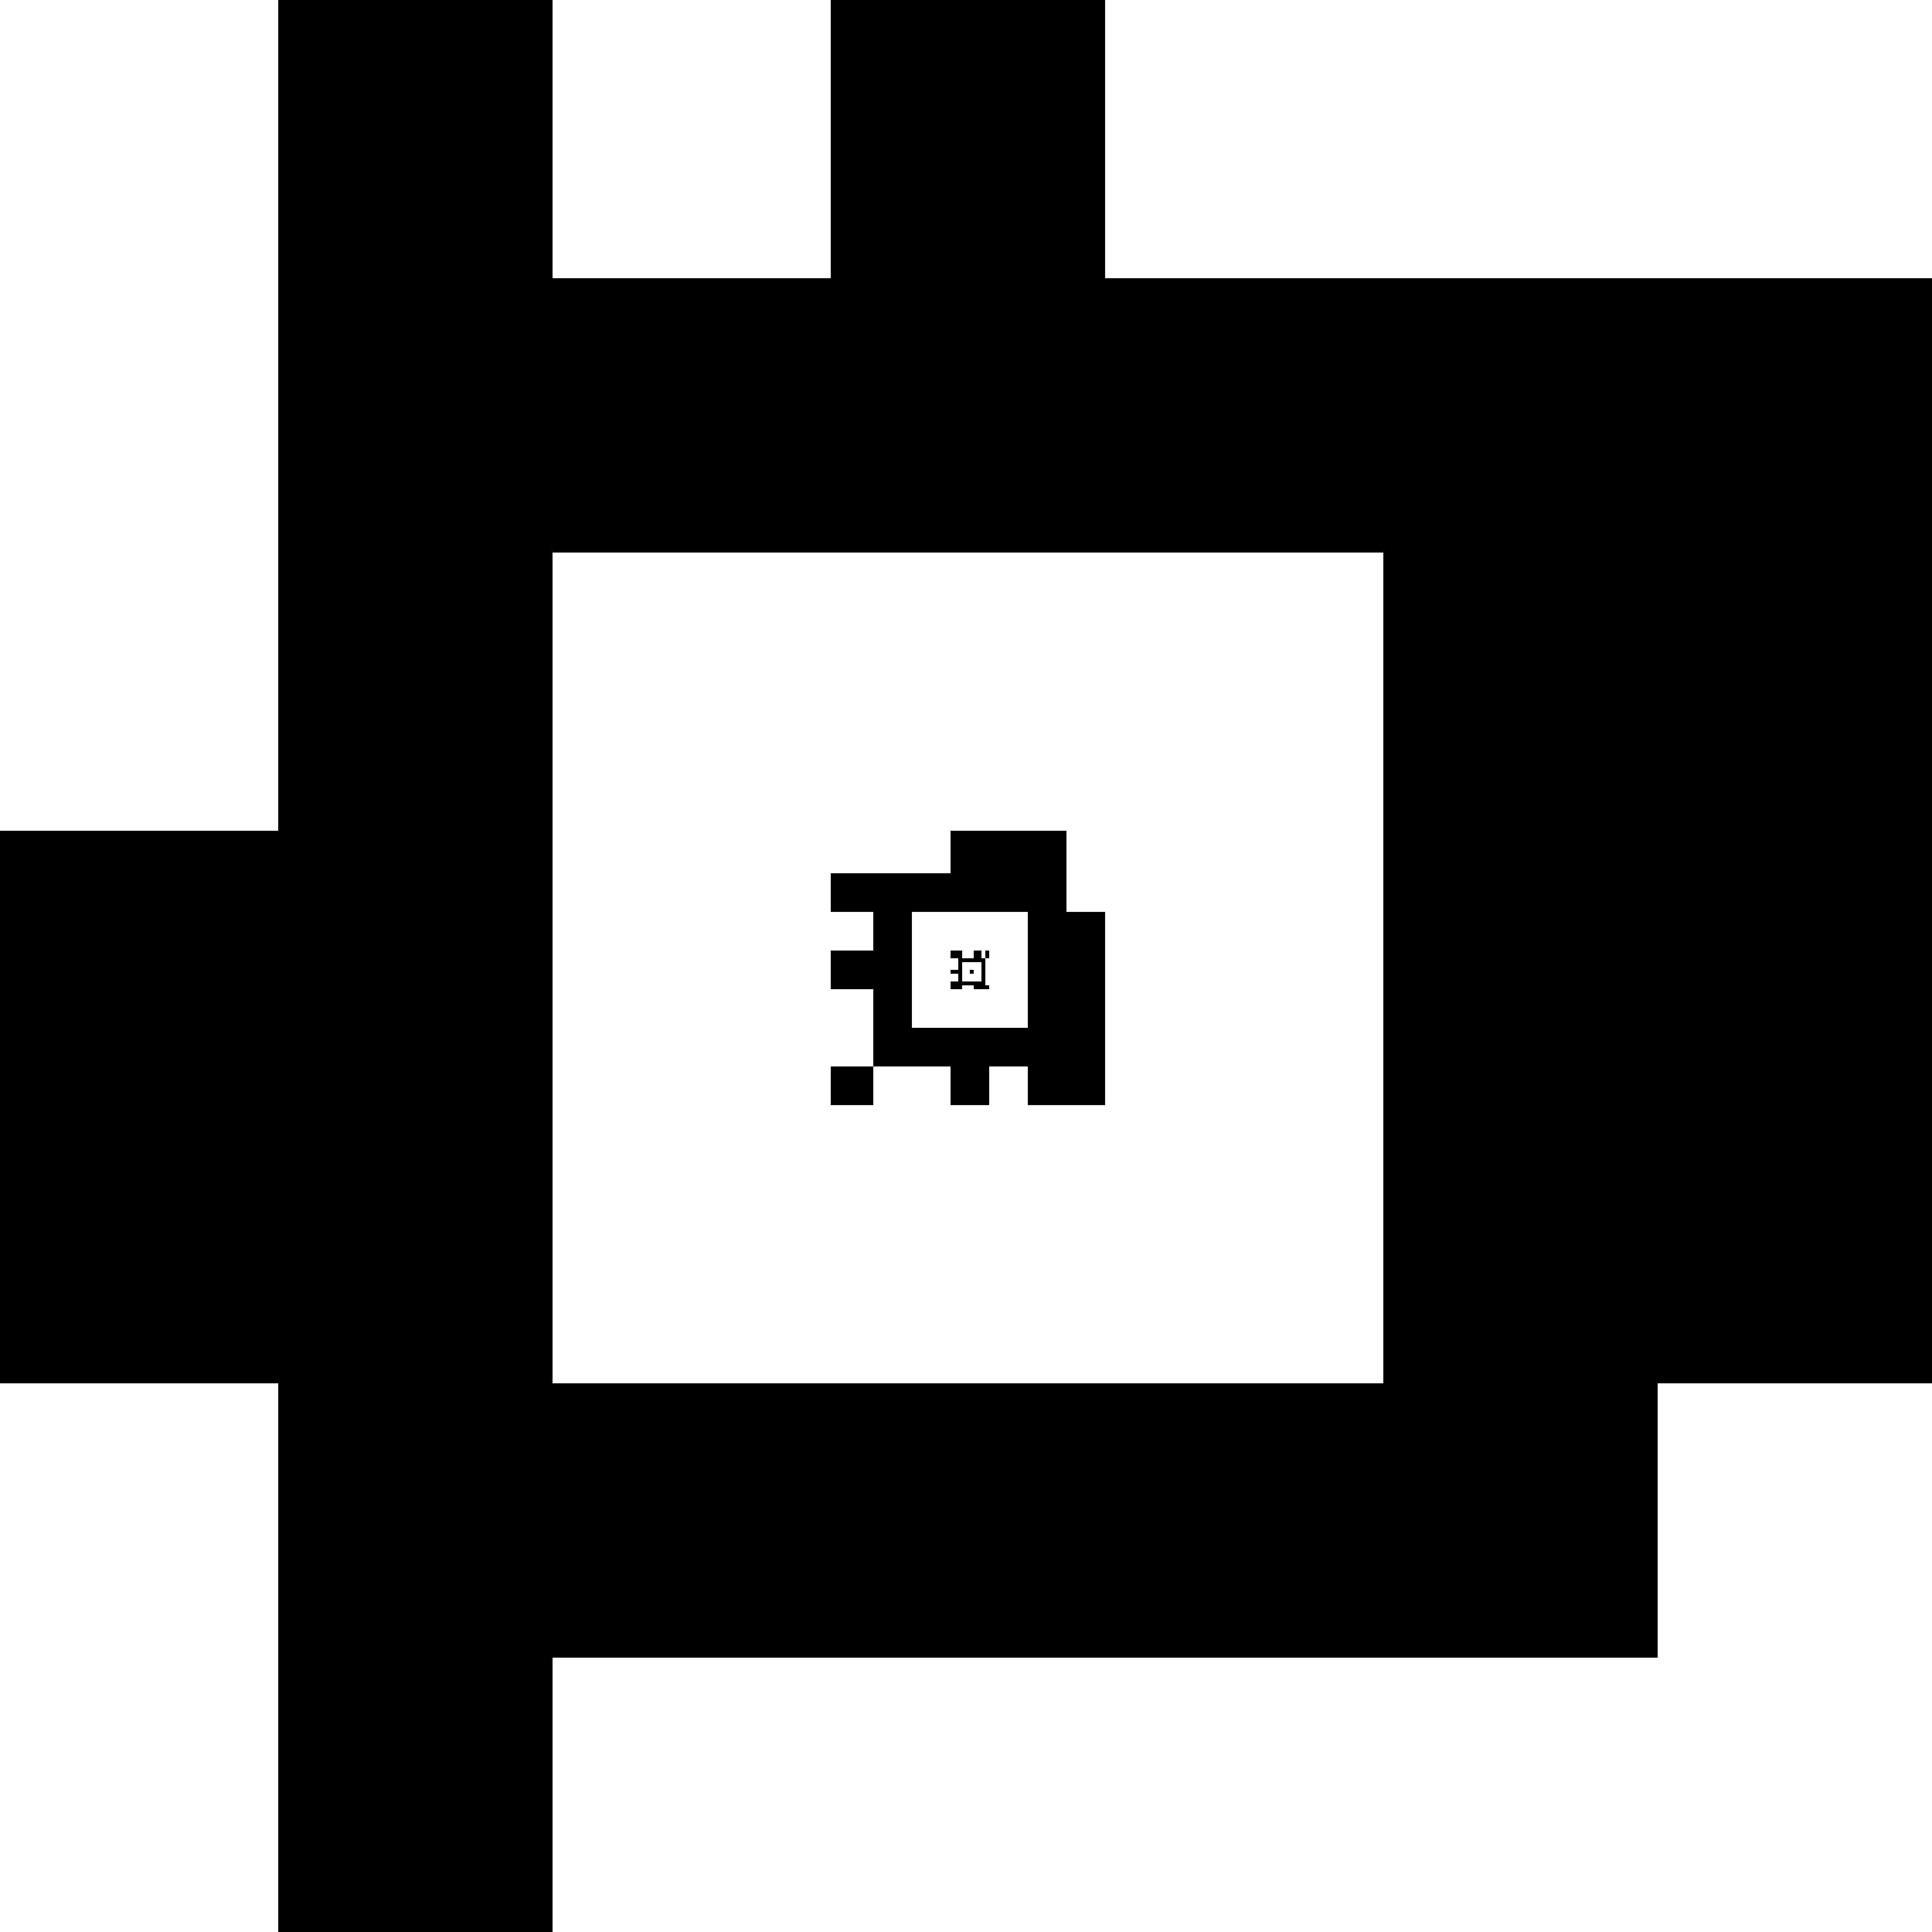
\includegraphics[width=5cm]{images/tagCustom24h10_00002_00001_00000}
      \caption{The landing pad with 3 embedded April Tags of the 24h10 family.}
    \end{figure}

  \end{block}

  \begin{alertblock}{System Design \& Equipment}

    \begin{figure}
      \centering
      
\includegraphics[width=\linewidth]{images/spark_architecture.drawio.png}
      \caption{System data flow.}
    \end{figure}

  \end{alertblock}

\end{column}

\separatorcolumn

\begin{column}{\colwidth}

  \begin{alertblock}{Results}

    Nullam non est elit. In eu ornare justo. Maecenas porttitor sodales lacus,
    ut cursus augue sodales ac.

    $$
    \int_{-\infty}^{\infty} e^{-x^2}\,dx = \sqrt{\pi}
    $$

    Interdum et malesuada fames $\{1, 4, 9, \ldots\}$ ac ante ipsum primis in
    faucibus. Cras eleifend dolor eu nulla suscipit suscipit. Sed lobortis non
    felis id vulputate.

    \heading{A heading inside a block}

    Praesent consectetur mi $x^2 + y^2$ metus, nec vestibulum justo viverra
    nec. Proin eget nulla pretium, egestas magna aliquam, mollis neque. Vivamus
    dictum $\mathbf{u}^\intercal\mathbf{v}$ sagittis odio, vel porta erat
    congue sed. Maecenas ut dolor quis arcu auctor porttitor.

    \heading{Another heading inside a block}

    Sed augue erat, scelerisque a purus ultricies, placerat porttitor neque.
    Donec $P(y \mid x)$ fermentum consectetur $\nabla_x P(y \mid x)$ sapien
    sagittis egestas. Duis eget leo euismod nunc viverra imperdiet nec id
    justo.

    \heading{Lipsum}
    \lipsum[50-51]

  \end{alertblock}

%  \begin{block}{Results}
%
%    Class aptent taciti sociosqu ad litora torquent per conubia nostra, per
%    inceptos himenaeos. Phasellus libero enim, gravida sed erat sit amet,
%    scelerisque congue diam. Fusce dapibus dui ut augue pulvinar iaculis.
%
%    \begin{table}
%      \centering
%      \begin{tabular}{l r r c}
%        \toprule
%        \textbf{First column} & \textbf{Second column} & \textbf{Third column} & \textbf{Fourth} \\
%        \midrule
%        Foo & 13.37 & 384,394 & \alpha \\
%        Bar & 2.17 & 1,392 & \beta \\
%        Baz & 3.14 & 83,742 & \delta \\
%        Qux & 7.59 & 974 & \gamma \\
%        \bottomrule
%      \end{tabular}
%      \caption{A table caption.}
%    \end{table}
%
%  \end{block}

  \begin{block}{References}

    \nocite{*}
    \footnotesize{\bibliographystyle{plain}\bibliography{poster}}

  \end{block}

\end{column}

\separatorcolumn
\end{columns}
\end{frame}

\end{document}
